\part{Resultados}

\chapter[Resultados]{Resultados}\label{Capitulo5}

Este trabalho resultou em uma aplicação web 2.0 que ajuda na fase interna de licitação através de uma melhoria de comunicação.
Para atingirmos essas melhorias, nós mapeamos os problemas e criamos as soluções.
Soluções essas, que foram pensadas com vistas à centralizar para o usuário, informações atualizadas sobre processos licitatórios.

A fim de centralizar essas informações foi necessário obter dados sobre as licitações e também sobre items, materiais, serviços e licitações, e vinculá-las ao nosso banco de dados
A obtenção desses dados é feita através de ação no sistema que recupera os dados na API de Compras Governamentais, forma pela qual o banco de dados pode se manter sempre atualizado com as licitações mais recentes.

Através dessa base de dados sempre atualizada, o usuário pode buscar na aplicação, o item pelo seu código ou descrição.
Sempre que há uma solicitação, cada setor de compras dos \textit{campi} recebem uma requisição informando sobre um processo licitatório iniciado.
Isso permite que um câmpus interessado em participar de um licitação iniciada por outro câmpus possa fazer sua adesão, indicando quais item, materiais ou serviços gostaria de comprar junto.

O sistema desenvolvido agiliza um processo burocrático, dando celeridade na troca de informações sobre compras inter-\textit{campi}.


\section{Disponibilidade do Sistema}

Os sistema está disponível no GitHub no endereço:~\url{https://github.com/dragao1995/licitacaoweb} sob a Licença Apache 2.0.

\begin{figure}[htbp]
	\centering
	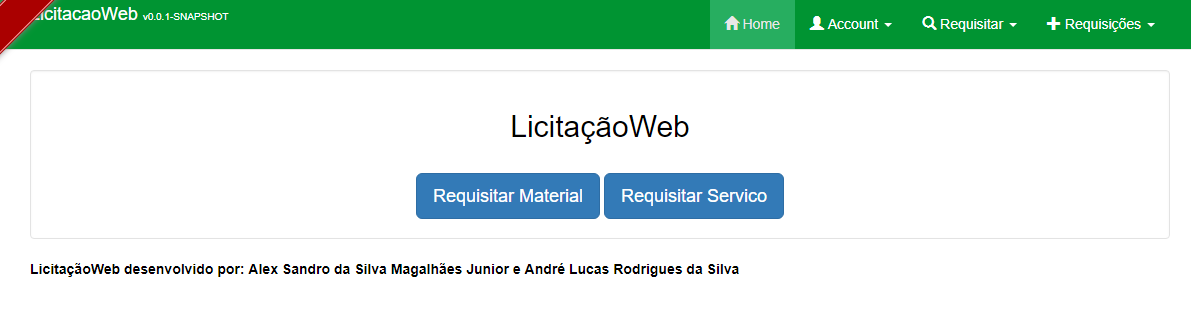
\includegraphics[width=0.95\textwidth]{figuras/prototipo001.png}
	\caption[Tela home LicitaçãoWeb]{Tela home LicitaçãoWeb.}
\end{figure}



